\chapter{Implementacja}
\label{cha:implementacja}

Ze względu na charakter aplikacji, która składa się z autonomicznych elementów, znaczna część implementacji poszczególnych serwisów mogła odbywać się niezależnie od innych. Tworzone funkcjonalności testowane były przy pomocy narzędzia Postman, za pomocą którego można wysyłać dowolnie skonfigurowane zapytania HTTP na konkretne adresy URI. Kolejne, gotowe usługi były następnie integrowane w sytemie.

%---------------------------------------------------------------------------

\section{Metodyka pracy}
Projekt powstawał iteracyjnie. To znaczy, że podczas pracy zaczynano od małych celów i po ich realizacji - stawiano trochę większe, udoskonalano obecny wówczas stan i przechodzono do kolejnego, bardziej zaawansowanego kroku. W ten sposób, możliwe było dokładne kontrolowanie rozwoju systemu, jego testowanie i w razie problemów, szybka analiza i znalezienie ich przyczyny. 

\subsection{Version Control System}
\textbf{VCS} - rozwój projektu śledzony był za pomocą systemu kontroli wersji.
Pozwala on dokumentować wszystkie, kolejne zmiany, które mają miejsce w odniesieniu do kodu. Dzięki temu wygodniejsze są również potencjalne eksperymenty, ponieważ w każdym momencie, możliwy jest powrót do dowolnego, poprzedniego stanu implementowanych funkcjonalności.\cite{vcs}


%---------------------------------------------------------------------------

\section{Wybór technologii}

%---------------------------------------------------------------------------

\section{Wielowątkowe tworzenie ofert}

%---------------------------------------------------------------------------

\section{Autoryzacja użytkownika w Allegro API}

Do integracji serwisu z aplikacją potrzebne jest pozyskanie tokenu dostępowego. Allegro udostępnia tzw. ``ścieżkę device flow``, dzięki której cały proces odbywa się bez konieczności uwzględniania go w interfejsie graficznym. Poniżej zaprezentowany jest diagram prezentujący tę funkcjonalność.\\

\begin{figure}[H]
	\centering
	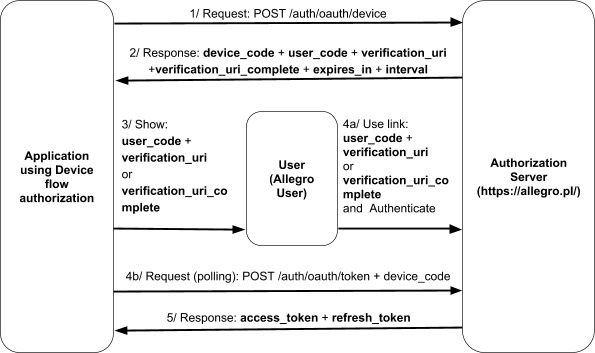
\includegraphics[width=\linewidth]{device_flow.png}
	\caption{Autoryzacja użytkownika typu Device flow}
	\caption*{Źródło: {https://developer.allegro.pl/}}
\end{figure}

Podejście w tej pracy zakłada zarejestrowanie jednego, wspólnego dla całego systemu, konta funkcjonalnego za pomocą którego każde zapytanie będzie autentykowane. Stwarza to niestety jedno ograniczenie, a mianowicie, ze względu na obowiązujący główny limit nakładany na Client ID po przekroczeniu liczby 9000 zapytań na minutę, aplikacja zwróci status HTTP 429 i zostanie zabklokowana na kolejne 60 sekund.\\
W fazie inicjalizacyjnej autoryzacji uzyskane zostaną dwa unikalne tokeny: 
\begin{itemize}
	\item dostępowy - ważny przez 12h.
	\item odświeżający - ważny 6 miesięcy.
\end{itemize}
Zostaną one zachowanie w pamięci, a każde kolejne zapytanie, w przypadku wygaśnięcia tokenu dostępowego, spowoduje jego odnowienie.
\begin{figure}[H]
	\centering
	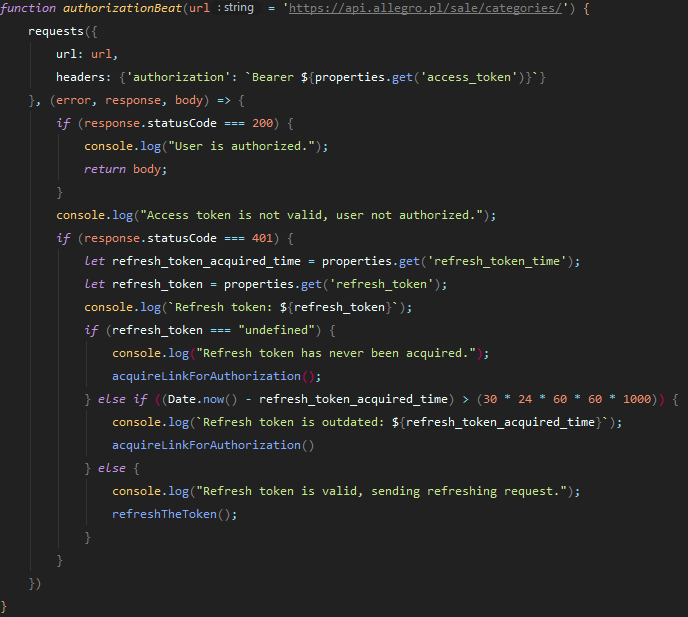
\includegraphics[width=\linewidth]{authorization.png}
	\caption{Kod odpowiedzialny za utrzymywanie ważnego tokena}
\end{figure}
Powyższy kod prezentuje przebieg akcji, które maja miejsce za każdym razem, kiedy otrzymywane jest zapytanie do OffersService(2.4). Na początku sprawdzane jest, czy token jest zwyczajnie aktualny, następnie, w przypadku, gdy nie jest, pobierany jest token odświeżający. W zależności od tego, czy jest on ważny, wygaśnięty, czy może w ogóle nigdy nie został uzyskany, odpowiednia logika zostaje uruchomiona.

%---------------------------------------------------------------------------


\section{Wdrożenie}

%---------------------------------------------------------------------------

\section{Elementy konifguracyjne}

%---------------------------------------------------------------------------